\chapter{Alternating Currents}

a \keypoint{direct current} (d.c.) flows in one direction only

an \keypoint{alternating current} (a.c.) reverses its flow direction from time to time

a.c. has certain advantages than d.c., as you will see in this chapter

we will study the mathematics of a.c. and the transmission process for a.c.

\subsection{sinusoidal a.c.}

as we have seen in \S\ref{subsection:generators}, currents produced from generators are naturally sinusoidal

sinusoidal a.c. is one of the most important types of a.c. waveform in electrical engineering.

for most cases in this course, we focus on a.c. that varies like a sine wave

\subsection{sinusoidal waveform}

\begin{marginfigure}
	\centering
	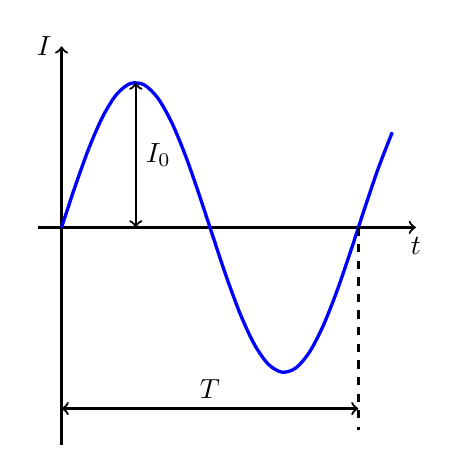
\begin{tikzpicture}[xscale=0.6,yscale=0.92]
	\draw [thick, ->] (-0.5,0) --(7.5,0) node[below]{$t$};
	\draw [thick, ->] (0,-3) --(0,2.5) node[left]{$I$};
	\draw [very thick,color=blue,domain=0:7,smooth,variable=\x] plot (\x,{2*sin(\x r)});
	\draw [thick,<->] (0,-2.5) -- (2*pi,-2.5) node[midway,above]{$T$};
	\draw [thick,dashed] (2*pi,0) -- (2*pi,-2.8);
	\draw [thick,<->] (pi/2,0) -- (pi/2,1) node[right]{$I_0$} -- (pi/2,2);
	\end{tikzpicture}
	
\end{marginfigure}

current: $\boxed{I = I_0 \sin \omega t}$ / voltage: $\boxed{V = V_0 \sin \omega t}$

\cmt $I_0$, $V_0$ are called \emph{peak current} and \emph{peak voltage} (amplitudes of the a.c. signal)

\cmt $\omega$ is \keypoint{angular frequency}\index{angular frequency}, which describes how fast a.c. signal oscillates (same idea as for simple harmonic motion, see \S\ref{section:oscillation})

frequency and period of the signal are given by:

{

\centering

$\omega = 2 \pi f$, $\,$ $T = \frac{1}{f} = \frac{2\pi}{\omega} $

}

\cmt mean current: $\avg{I} = 0$, mean voltage: $\avg{V}=0$

this is because a.c. signal fluctuates with time, positive and negative bits cancel out

\newpage

\question{An alternating voltage has a peak value of 16 V and period of 0.10 s. Write down a mathematical equation that describes the variation of this voltage.}

\question{An alternating voltage is produced from a simple generator. If the rotating speed of the coil in the generator doubles, describe quantitatively the change in the peak value and frequency of the alternating voltage.}

\question{A student argues that when an alternating current is driven through a resistor, the mean current is zero, so an alternating current does not produce heating power on the resistor. State and explain whether this is correct.}




\subsection{power}

electrical power dissipated in a resistor: $P = I^2 R$, or, $P=\frac{V^2}{R}$

since $I^2, V^2 \geq 0$, $P$ can never be negative, so an a.c. can produce effective power in a resistor

note that for an a.c., $P$ keeps changing with time, as $I$ and $V$ are both varying with time

in everyday life, we are more concerned about the \emph{mean power}

mean power output for an a.c. is: $\avg{P} = \avg{I^2} R = \frac{\avg{V^2}}{R}$

so we see the necessity to introduce mean square values $\avg{I^2}$  and $\avg{V^2}$

let's further introduce root mean square (r.m.s.) values: $I_\text{rms} = \sqrt{\avg{I^2}}$, and $V_\text{rms} = \sqrt{\avg{V^2}}$

we can now write the mean power for a.c. as: $\boxed{\avg{P} = I^2_\text{rms} R = \frac{V^2_\text{rms}}{R}}$

\begin{marginfigure}
	\centering
	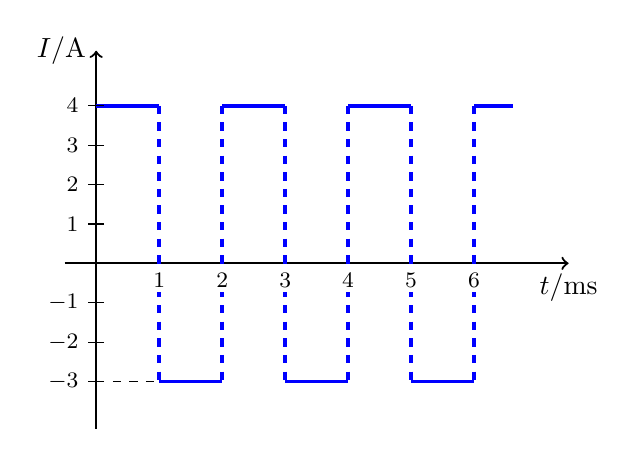
\begin{tikzpicture}
		\draw [thick, ->] (-0.4,0) --(6,0) node[below]{$t$/ms};
		\draw [thick, ->] (0,-2.1) --(0,2.7) node[left]{$I$/A};
		\foreach \x in {0,1.6,3.2}
		{
			\draw [very thick,blue] (\x,2) --++ (0.8,0);
			\draw [very thick,blue] (\x+0.8,-1.5) --++ (0.8,0);
			\draw [very thick,blue, dashed] (\x+0.8,2) -- (\x+0.8,-1.5);
			\draw [very thick,blue, dashed] (\x+1.6,2) -- (\x+1.6,-1.5);
		}
		\draw [very thick,blue] (4.8,2) --++ (0.5,0);
		\foreach \y in {-3,-2,-1,1,2,3,4} \draw(0.1,\y/2) --++ (-0.2,0) node[left]{\footnotesize $\y$};
		\draw [dashed] (0,-1.5) --++ (0.8,0);
		\foreach \x in {1,2,3,4,5,6}
		{
			\draw[white,fill] (\x*0.8-0.1,-0.36) rectangle (\x*0.8+0.1,-0.02);
			\node[below] at (\x*0.8,0) {\footnotesize $\x$};
		}
	\end{tikzpicture}
\end{marginfigure}

\example{The variation with time of an alternating current in a resistor of $120 \Omega$ is shown. (a) What is the value of its r.m.s. current? (b) What is the mean power dissipated by the resistor?}

\sol $\avg{I^2} = \frac{4^2+(-3)^2}{2} = 12.5 \text{ A}^2$

$I_\text{rms} = \sqrt{\avg{I^2}} = \sqrt{12.5} \approx 3.54 \text{ A}$

$\avg{P} = I_\text{rms}^2 R = 12.5 \times 120 = 1500 \text{ W}$ \eoe

\subsection{r.m.s. current \& r.m.s. voltage}

in last section, we studied the mathematical aspect of the r.m.s. value

but we still need a definition for r.m.s. current and r.m.s. voltage from a physical viewpoint

physically, r.m.s. value of an alternating current is defined as follows

\begin{ilight}
	\keypoint{r.m.s. current/voltage}\index{r.m.s. current}\index{r.m.s. voltage} of an a.c. equals a steady d.c. current/voltage that delivers same average power to a resistive load
\end{ilight}

\eqyskip

\cmt for \emph{sine waves}, r.m.s values are related to peak values by: $\boxed{I_\text{r.m.s} = \frac{1}{\sqrt{2}}I_0}$ and $\boxed{V_\text{r.m.s} = \frac{1}{\sqrt{2}}V_0}$

\begin{compactenum}
	\item[proof:] total energy dissipation in one period is: $W_T = \int^T_0 P \dd  t$
	
	\eqyskip
	
	so mean power can be given by: $\avg{P} = \frac{W_T}{T} = \frac{1}{T} \int^T_0 P \dd t$
	
	\eqyskip
	
	substitute $P=I^2 R \xlongequal{I=I_0\sin\omega t} I^2_0 R \sin^2 \omega t$, we have: $\avg{P} = \frac{I^2_0 R}{T} \int^T_0 \sin^2 \omega t \dd t$
	
	\eqyskip
	
	the integral is carried out: $\int^T_0 \sin^2 \omega t \dd t = \frac{1}{2} \int_0^T (1-\cos2 \omega t) \dd t = \frac{1}{2} \Big(t - \frac{\sin \omega t}{2\omega} \Big) \Bigg|_0^T = \frac{1}{2}$
	
	\eqyskip
	
	now we have: $\avg{P} = I_\text{rms}^2 R = \frac{1}{2} I_0^2 R \RA I_\text{rms} = \frac{1}{\sqrt{2}} I_0$
	
	a similar calculation for voltage would show: $V_\text{rms} = \frac{1}{\sqrt{2}} V_0$  \eoe
\end{compactenum}

\cmt it is worth pointing out that the $\tfrac{1}{\sqrt{2}}$-relation for r.m.s. values only holds for sine waves

for other waveforms, e.g., square waves or triangle waves, numerical constant is different

\cmt value of voltages stated for mains electricity supply usually refers to the r.m.s. value\footnote{Different countries have different standards. For example, China mains electricity supplies a voltage of 220 V. UK uses a 230 V distribution system. USA has national standard of a 110 V voltage. These are all r.m.s. voltages.}

\example{An a.c. power supply produces a sinusoidal output across a resistor of 30 $\Omega$. The maximum voltage is found to be 75 V. Find energy dissipated in the resistor in 2.0 minutes.}

\sol r.m.s voltage: $V_\text{rms} = \frac{1}{\sqrt{2}} V_0 = \frac{75}{\sqrt{2}} \approx 53.0 \text{ V}$

\eqyskip

mean power output: $\avg{P} = \frac{V^2_\text{rms}}{R} = \frac{53.0^2}{30} \approx 93.8 \text{ W}$

energy dissipation: $W = \avg{P} t = 93.8 \times 2.0 \times 60 \approx 1.13 \times 10^4 \text{ J}$ \eoe

\newpage

\question{An alternating voltage $V$ is represented by the equation: $ V = 310 \sin(100\pi t)$, where $V$ and $t$ are measured in SI units. For this voltage, find (a) the peak voltage, (b) the r.m.s voltage, (c) the frequency, (d) the mean power when it is applied across a resistor of 250 $\Omega$.}

\question{What is the average power dissipated in a resistor when the alternating supply has a peak current of 5.0 A and a peak voltage of 8.0 V?}

\question{The peak value of a sinusoidal alternating current is equal to a steady direct current. When they are applied to the same load, what is the ratio of power dissipation $\frac{P_\text{d.c.}}{P_\text{a.c.}}$?}

\subsection{measurement of a.c. with an oscilloscope}

to measure a varying voltage, we can use a \keypoint{cathode-ray oscilloscope} (c.r.o.) \index{oscilloscope} (see figure\footnote{The illustration of the oscilloscope was created by \emph{Hugues Vermeiren}. The source code is downloaded from TeXample: \url{http://www.texample.net/tikz/examples/textronics-oscilloscope/}.  })

\begin{center}
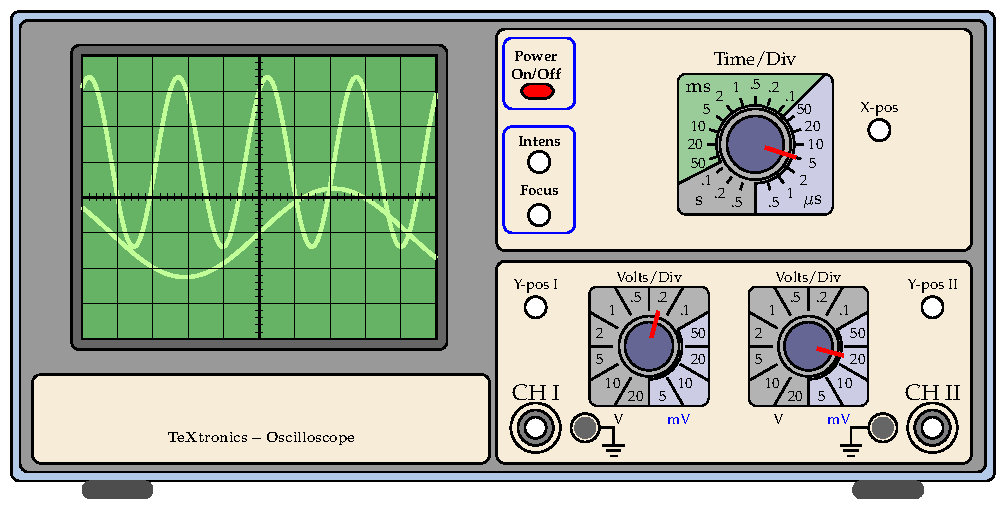
\includegraphics[height=190pt]{oscilloscope.pdf}
\end{center}

an oscilloscope is basically an electron deflection tube that uses a beam of electrons to trace the input voltage as a function of time.

electron beam is controlled by two sets of parallel plates

horizontal plates control how fast beam moves across screen, giving a horizontal time axis

a.c. voltage is applied across vertical plates, causing beam to bend upwards or downwards

when beam hits fluorescent screen, entire trace of the beam can be seen across the screen

\cmt to take readings from oscilloscope, remember it displays a voltage against time graph

\begin{compactenum}
	\item[-] \keypoint{voltage gain}, or \keypoint{Y-gain}, tells the number of volts per vertical division
	
	\item[-] \keypoint{time base} gives the time unit per horizontal division
\end{compactenum}




\example{An oscilloscope displays an a.c. voltage signal as shown.}\label{ex-readcro}

\begin{marginfigure}
\centering
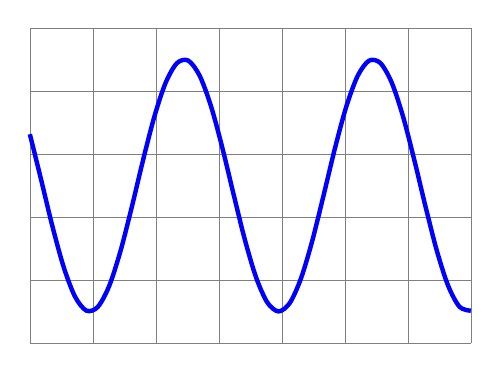
\begin{tikzpicture}[scale=0.8]
\draw[style=help lines,step=1] (0,-3) grid (7,2);
\draw [ultra thick,color=blue,domain=0:7,samples=40,smooth,variable=\x] plot (\x,{2*sin(((\x- 1.7)*2*pi/3 ) r) -0.5 });
\end{tikzpicture}
\end{marginfigure}

suppose the time base setting is $10$ ms/div, and the voltage gain is $5$ V/div.
 
4 vertical divisions from highest to lowest, so

\eqskip peak voltage: $V_0= \frac{1}{2} \times 4 \times 5 = 10 \text{ V}$

3 horizontal divisions between peak to peak, so

\eqskip period: $T = 3 \times 10 = 30 \text{ ms}$
	
\eqskip frequency $f = \frac{1}{T} = \frac{1}{30\times10^{-3}} \approx 33.3 \text{ Hz} $ \eoe



\question{In Example \ref{ex-readcro}, if the time-base setting is 5 ms/div and the voltage gain is 2 V/div, write down an equation that represents this alternating voltage.}



\subsection{power supply systems}

\subsection{high-voltage transmission}

electricity is sent from power stations to consumers around the country

for long-distance transmission, we need minimise energy losses 

power dissipated due to resistance in cables is $I^2 R$, should transmit at low currents

since output power of a power station is fixed, low current means high voltage

so transmission at high voltages minimises energy loss in power grids

but for reasons of safety and efficiency, desirable to have low voltages at both generating end (power station) and receiving end (home or factory)

this requires converting a.c. into higher or lower voltages $\ra$ need for \emph{transformers}

\begin{figure}[ht]
	\centering
	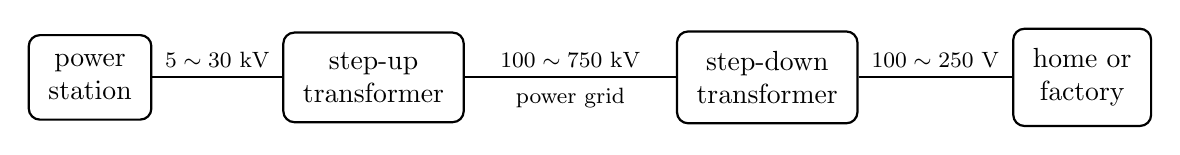
\begin{tikzpicture}[force/.style={align=center,execute at begin node=\setlength{\baselineskip}{1.2em},draw,thick,rounded corners,inner sep=.25cm}]
	
	\node [force] (powerstation) at (0,0) {power\\station};
	\node [force] (step-up) at (3.6,0) {step-up\\transformer};
	\node [force] (step-down) at (8.6,0) {step-down\\transformer};
	\node [force] (home) at (12.6,0) {home or\\factory};
	
	\draw[thick] (powerstation) to node[midway,above]{\footnotesize $5\sim30$ kV} (step-up) to node[midway,above]{\footnotesize $100\sim750$ kV} node[midway,below]{\footnotesize power grid} (step-down) to node[midway,above]{\footnotesize $100\sim250$ V} (home);
	
	\end{tikzpicture}
\end{figure}

\subsection{transformers}  \label{subsection:transformers}

\keypoint{transformer}\index{transformer} is a device that can change values of voltage for an alternating current

transformers are an important part of the national power grid

transformers are essential for transmission, distribution, and utilization of electrical energy


\begin{figure}[ht]
	\centering
\begin{tikzpicture}[scale=1.35]
\draw[thick,rounded corners,fill=gray!15] (-2,-2.2) rectangle (2,2.2);
\draw[thick,rounded corners,fill=white] (-1.2,-1.4) rectangle (1.2,1.4);
\draw[very thick] (-3.2,1) -- (-1.2,1) (1.2,1) -- (3.2,1);
\draw[very thick] (-3.2,-1) -- (-1.2,-1) (1.2,-1) -- (3.2,-1);
\foreach \x in {0.95,0.85,...,-0.95} \draw[very thick] (-2,\x) -- ++ (0.8,-0.05);
\foreach \x in {0.95,0.75,...,-0.95} \draw[very thick] (1.2,\x) -- ++ (0.8,-0.05);
\draw[very thick,<->] (-2.8,1) node[above]{input} -- (-2.8,0) node[left]{$V_p$} --(-2.8,-1);
\draw[very thick,<->] (2.8,1) node[above]{output} -- (2.8,0) node[right]{$V_s$} --(2.8,-1);
\draw[thick] (-1.6,-1.1) -- (-2.5,-2.4) node[below,twoline]{primary\\coil};
\draw[thick] (1.6,-1.1) -- (2.5,-2.4) node[below,twoline]{secondary\\coil};
\draw[thick] (0,1.8) -- (1,2.7) node[right]{iron core};
\end{tikzpicture}

structure of a typical transformer
\end{figure}

\cmt principle of transformers

a.c. flowing in \keypoint{primary coil} (input) produces a changing magnetic field, i.e. a changing flux

this flux is linked with \keypoint{secondary coil} through iron core

an a.c. voltage with same frequency is then induced in secondary coil (output)

\cmt \keypoint{turns-ratio equation} for a transformer

assume no loss in magnetic flux, i.e., all field inside transformer's iron core

from Faraday's law: $V_p = N_p \frac{\dd \phi}{\dd t}$, $V_s = N_s \frac{\dd \phi}{\dd t}$, where $N_p$, $N_s$ are number of turns of coils

\eqyskip cancel out $\frac{\dd \phi}{\dd t}$, we find: $\boxed{ \frac{V_s}{V_p} = \frac{N_s}{N_p} }$



\xskip 
if $N_p < N_s$, output voltage is increased $\,\rightarrow\,$ \emph{step-up transformers}

if $N_p > N_s$, output voltage is decreased $\,\rightarrow\,$ \emph{step-down transformers}

\cmt if transformer is 100\% efficient, then input power equals output power

for ideal transformers: $\boxed{I_p V_p  = I_s V_s} $

\cmt in practice, there always exists losses of energy from the transformer

causes of energy loss from the transformer include

\begin{compactitem}
\item[-] heat produced by \emph{eddy currents} induced in iron core

this is reduced by \emph{laminating} the core with insulate layers

\item[-] heat generated in coils due to resistance

can use thick copper wire to minimise resistance

\item[-] leakage of magnetic flux into surroundings

transformer's core is made of a continuous loop of iron to minimise this effect

\end{compactitem}

\example{An ideal transformer has 200 turns on the primary coil and 5000 turns on the secondary	coil. The r.m.s. input voltage to the primary coil is 8.0 V. What is the \emph{peak} voltage across a resistor connected to the secondary coil?}

\solc\begin{equation*}
\frac{V_{s,0}}{V_{p,0}} = \frac{N_s}{N_p} \RA 
\frac{V_{s,0}}{\sqrt{2}V_{p,\text{rms}}} = \frac{N_s}{N_p} \RA
\frac{V_{s,0}}{8.0\times\sqrt{2}} = \frac{5000}{200} \RA
V_{s,0} \approx 2830 \text{ V}   
\end{equation*}

\question{An ideal transformer has 6000 turns on its primary coil. It converts a mains supply of 220 V r.m.s. to an a.c. voltage with a peak value of 12.0 V. Find the number of turns on the secondary coil.}

\question{If a \emph{steady} d.c. voltage is applied to the input of a simple transformer, what is the output voltage produced?}

\question{State and explain whether the current in the primary coil of a transformer is in \emph{phase} with the voltage induced in the secondary coil.}

\subsection{rectifiers}

some electronic equipments (e.g., your smartphone, laptop, etc.) must work with d.c.

for these appliances require \keypoint{rectification}\index{rectification}, a process that converts an a.c. into a d.c.

rectification uses \emph{diodes}\index{diode}, electronic components that only allow current in one direction

\subsection*{half-wave rectification}\index{rectification!half-wave rectification}


half-wave rectification uses a single diode

\begin{figure}[ht]
	\centering
	\begin{minipage}{0.4\linewidth}
			\centering
			\begin{circuitikz}[xscale=1,yscale=1.1,european resistors]
				\draw (0,0) to[sV,l^=$V_\text{in}$] (0,3) to[Do] (3,3) to[R,l_=$R$] (3,0) -- (0,0);
				\draw (3,3) -- (4.2,3) (3,0) -- (4.2,0);
				\draw[<->] (3.8,0) --++ (0,3) node[right,midway]{$V_\text{out}$};
				\node[right] at (0,2.2) {$X$};
				\node[right] at (0,0.8) {$Y$};
				\node[right] at (3,2.4) {$P$};
				\node[right] at (3,0.6) {$Q$};
			\end{circuitikz}
		\end{minipage}\hfil
	\begin{minipage}{0.54\linewidth}
		\centering
		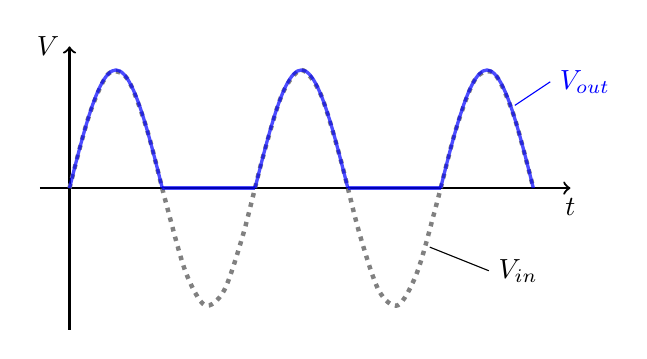
\begin{tikzpicture}[xscale=0.75,yscale=1.5]
		\draw [thick, ->] (-0.5,0) --(2.7*pi,0) node[below]{$t$};
		\draw [thick, ->] (0,-1.2) --(0,1.2) node[left]{$V$};
		\draw[ultra thick, dotted, gray, domain=0:2.5*pi,smooth,variable=\x] plot (\x,{sin(2*\x r)});
		\foreach \i in {0,1,2}
		\draw [very thick,opacity=0.7,blue,domain=\i*pi:(\i+0.5)*pi,smooth,variable=\x] plot (\x,{sin(2*\x r)});
		\draw [very thick, opacity=0.7,blue] (0.5*pi,0) -- (pi,0) (1.5*pi,0) -- (2*pi,0);
		\draw (6.1,-0.5) --++ (1,-0.2) node[right]{$V_\text{in}$};
		\draw[blue] (2.4*pi,0.7) --++ (0.6,0.2) node[right]{$V_\text{out}$};
		\end{tikzpicture}
		
	\end{minipage}
\end{figure}

when input terminal $X$ is positive, current can flow through diode, terminal $P$ is positive with respect to $Q$ for load resistor $R$ 

when input terminal $Y$ is negative, flow of current is blocked, so zero output voltage on $R$

$V_\text{out}$ across load $R$ is in one direction only, i.e., it becomes a d.c.

but power available from half-wave rectifier is only half of supply power

\subsection*{full-wave rectification}\index{rectification!full-wave rectification}

full-wave rectification requires using a combination of four-diode bridge structure

\begin{figure}[ht]
	\centering
	\begin{circuitikz}[scale=1.2,european resistors]
		\draw (0,-2) -- (-3.2,-2) to[sV,l^=$V_\text{in}$] (-3.2,2) -- (0,2);
		\draw (-2,0) to[Do] (0,2) to[Do] (2,0);
		\draw (-2,0) to[Do] (0,-2) to[Do] (2,0);
		\foreach \r in {1.35} \draw (-\r,\r) node{$A$} (\r,\r) node{$B$} (\r,-\r) node{$C$} (-\r,-\r) node{$D$};
		\draw[fill] (0,2) circle (0.05) (0,-2) circle (0.05) (2,0) circle (0.05) (-2,0) circle (0.05);
		\draw (-2,0) -- (-2,-3) -- (3,-3) to[R,l^=$R$] (3,0) -- (2,0);
		\draw (3,-3) -- (4.2,-3) (3,0) -- (4.2,0);
		\draw[<->] (3.8,0) --++ (0,-3) node[right,midway]{$V_\text{out}$};
		\node[right] at (-3.2,0.7) {$X$};
		\node[right] at (-3.2,-0.7) {$Y$};
		\node[right] at (3,-0.6) {$P$};
		\node[right] at (3,-2.4) {$Q$};
	\end{circuitikz}
\end{figure}

when input terminal $X$ is positive, current flow: $X \to B \to R \to D \to Y $

when input terminal $Y$ is positive, current flow: $Y \to C \to R \to A \to X $

either case, resulting output current in load resistor $R$ always flows in same direction

terminal $P$ is always positive with respect to $Q$ for $R$ no matter what polarity for $V_\text{in}$

output voltage across $R$ is now full-wave rectified


\begin{figure}[ht]
\centering
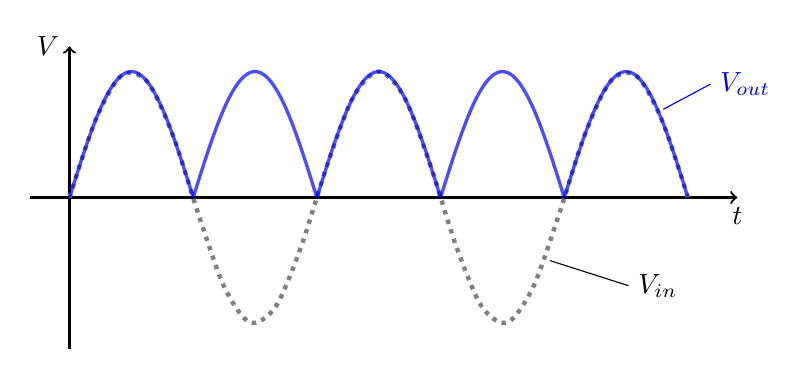
\begin{tikzpicture}[xscale=1,yscale=1.6]
\draw [thick, ->] (-0.5,0) --(2.7*pi,0) node[below]{$t$};
\draw [thick, ->] (0,-1.2) --(0,1.2) node[left]{$V$};
\draw[ultra thick, dotted, gray, domain=0:2.5*pi,smooth,variable=\x] plot (\x,{sin(2*\x r)});
\foreach \i in {0,1,2}
\draw [very thick, blue, opacity=0.7, domain=\i*pi:(\i+0.5)*pi, smooth, variable=\x] plot (\x,{sin(2*\x r)});
\foreach \i in {0.5,1.5}
\draw [very thick, blue, opacity=0.7, domain=\i*pi:(\i+0.5)*pi, smooth, variable=\x] plot (\x,{-sin(2*\x r)});
\draw (6.1,-0.5) --++ (1,-0.2) node[right]{$V_\text{in}$};
\draw[blue] (2.4*pi,0.7) --++ (0.6,0.2) node[right]{$V_\text{out}$};
\end{tikzpicture}
\end{figure}

\question{If we want to have terminal $Q$ to be positive with respect to $P$ for load resistor $R$, how should we rebuild the bridge rectifier with the same four diodes?}


\subsection{smoothing}

note that d.c. resulting from rectification still varies with time

to produce steady d.c. from fluctuating d.c., a process called \keypoint{smoothing}\index{smoothing} is carried out

smoothing uses \emph{capacitors}\index{capacitor}, which are connected in \emph{parallel} with the load resistor (see figure)

\begin{figure}[ht]
	\centering
	\begin{circuitikz}[scale=0.95,european resistors]
		\draw (0,-2) -- (-3,-2) to[sV,l^=$V_\text{in}$] (-3,2) -- (0,2);
		\draw (-2,0) to[Do] (0,2) to[Do] (2,0);
		\draw (-2,0) to[Do] (0,-2) to[Do] (2,0);
		\draw[fill] (0,2) circle (0.08) (0,-2) circle (0.08) (2,0) circle (0.08) (-2,0) circle (0.08);
		\draw (-2,0) -- (-2,-3) -- (3,-3) to[R,l^=$R$] (3,0) -- (2,0);
		\draw (3,-3) -- (4.5,-3) to[C,l^=$C$] (4.5,0) -- (3,0);
		\draw (4.5,-3) -- (6,-3) (4.5,0) -- (6,0);
		\draw[<->] (5.5,-3) -- (5.5,-1.5) node[right]{$V_\text{out}$} -- (5.5,0);
	\end{circuitikz}
\end{figure}

capacitor can store electrical energy as voltage output from rectifier rises

as voltage from rectifier drops, capacitor slowly discharges and feeds energy to the load 

output voltage $V_\text{out}$ across load will have less ripples over the cycles

less fluctuation in $V_\text{out}$ so we say $V_\text{out}$ is now smoothed

\begin{figure}[ht]
	\centering
\begin{tikzpicture}[xscale=1.35,yscale=2.7]
\draw [thick, ->] (-0.2,0) --(2.2*pi,0) node[below]{$t$};
\draw [thick, ->] (0,-0.2) --(0,1.2) node[left]{$V$};
\foreach \i in {0,1} {
\draw [very thick,blue,domain=(\i+0.16)*pi:(\i+0.25)*pi,smooth,variable=\x] plot (\x,{sin(2*\x r)});
\draw [thick, dashed,gray,domain=\i*pi:(\i+0.5)*pi,smooth,variable=\x] plot (\x,{sin(2*\x r)});
}
\foreach \i in {0.5,1.5} {
\draw [very thick,blue,domain=(\i+0.16)*pi:(\i+0.25)*pi,smooth,variable=\x] plot (\x,{-sin(2*\x r)});
\draw [thick, dashed,gray,domain=\i*pi:(\i+0.5)*pi,smooth,variable=\x] plot (\x,{-sin(2*\x r)});
}

\foreach \i in {0,0.5,1,1.5} 
\draw [very thick,blue] (\i*pi+0.25*pi,1) [out=-10,in=175] to (\i*pi+0.66*pi,0.844);

\draw [very thick,blue] (0,0.9) [out=-7,in=175] to (0.16*pi,0.844);
\draw (2*pi-0.1,0.4) --++ (0.8,0.1) node[right,twoline]{$V_\text{out}$ without\\smoothing};
\draw[blue] (2*pi,0.95) --++ (0.6,0.2) node[right,twoline]{$V_\text{out}$ after\\smoothing};
\end{tikzpicture}
\end{figure}

\cmt effect of smoothing is controlled by choice of load resistor $R$ and smoothing capacitor $C$

rate of charging and discharging depend on \emph{time constant} $RC$ (see \S\ref{sec:charging-capacitors})

greater $RC$, smoothing capacitor discharges more slowly, giving less ripples

a larger capacitor for a fixed resistor usually gives better smoothing effect

but if $RC$ is too large, charging would become very slow, capacitor might not be completely charged after each cycle, this could also result into undesirable effects

\question{If a second capacitor is added in \emph{series} with the first smoothing capacitor, use sketches to show the changes you would expect for the output voltage.}